\documentclass[]{standalone}

\usepackage{tikz}
\usepackage{arev}
\usepackage{arevmath}
\usepackage{arevtext}
  

\begin{document}
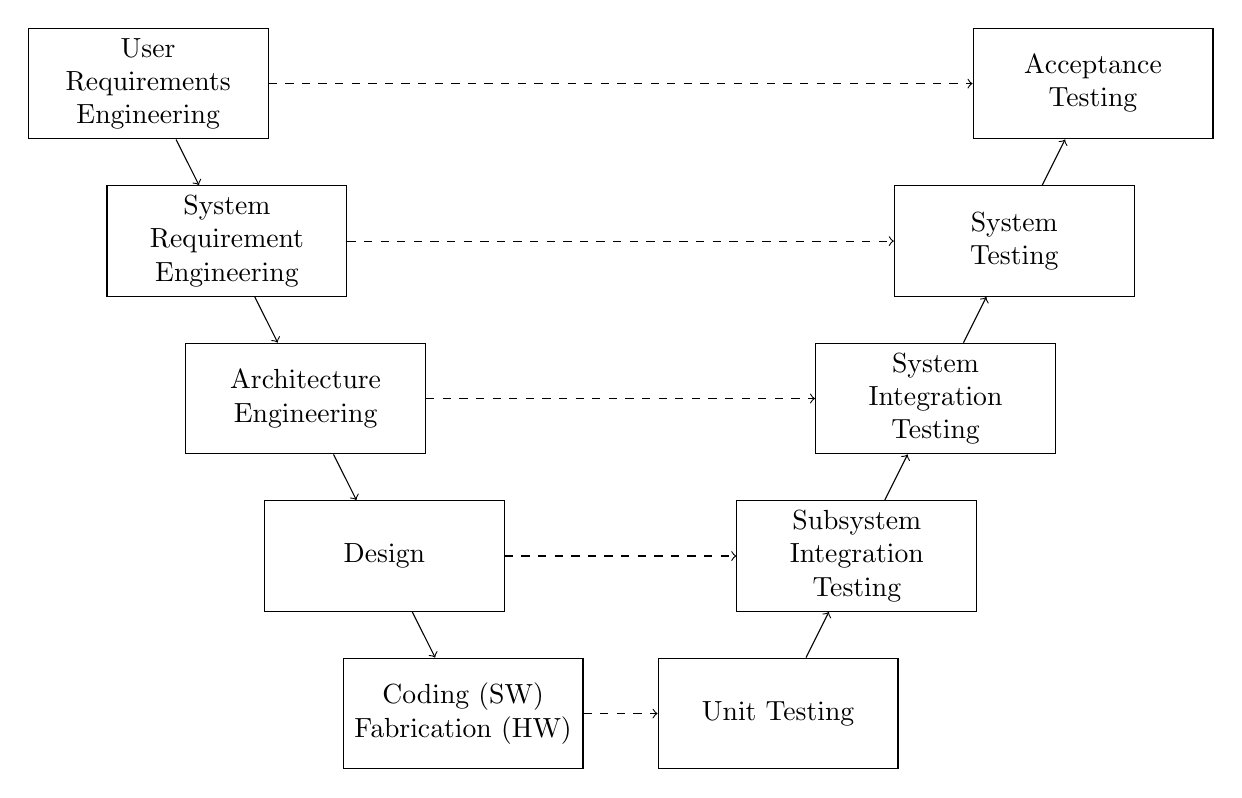
\begin{tikzpicture}[]
  \node[align=center, draw, text width=80, minimum height=40] (A) at (0,0) {User\\ Requirements\\ Engineering};
  \node[align=center, draw, text width=80, minimum height=40] (B) at (1,-2) {System\\ Requirement\\ Engineering};
  \node[align=center, draw, text width=80, minimum height=40] (C) at (2,-4) {Architecture\\ Engineering};
  \node[align=center, draw, text width=80, minimum height=40] (D) at (3,-6) {Design};
  \node[align=center, draw, text width=80, minimum height=40] (E) at (4,-8) {Coding (SW)\\ Fabrication (HW)};

  \node[align=center, draw, text width=80, minimum height=40] (F) at (12,0) {Acceptance Testing};
  \node[align=center, draw, text width=80, minimum height=40] (G) at (11,-2) {System\\ Testing};
  \node[align=center, draw, text width=80, minimum height=40] (H) at (10,-4) {System\\ Integration\\ Testing};
  \node[align=center, draw, text width=80, minimum height=40] (J) at (9,-6) {Subsystem\\ Integration\\ Testing};
  \node[align=center, draw, text width=80, minimum height=40] (K) at (8,-8) {Unit Testing};

  \draw[->] (A) -- (B);
  \draw[->] (B) -- (C);
  \draw[->] (C) -- (D);
  \draw[->] (D) -- (E);

  \draw[->, dashed] (E) -- (K);

  \draw[<-] (F) -- (G);
  \draw[<-] (G) -- (H);
  \draw[<-] (H) -- (J);
  \draw[<-] (J) -- (K);

  \draw[->, dashed] (D) -- (J);
  \draw[->, dashed] (C) -- (H);
  \draw[->, dashed] (B) -- (G);
  \draw[->, dashed] (A) -- (F);

\end{tikzpicture}
\end{document}